\documentclass{article}

\usepackage[utf8]{inputenc}
\usepackage[T1]{fontenc}
\usepackage{lmodern}
\usepackage{graphicx}
\usepackage{color}
\usepackage{hyperref}
\usepackage{amsmath}
\usepackage{amsfonts}
\usepackage{epstopdf}
\usepackage[table]{xcolor}
\usepackage{matlab}

\sloppy
\epstopdfsetup{outdir=./}
\graphicspath{ {./Lab01_images/} }

\begin{document}

\matlabtitle{LAB 1: INTRODUCTION TO MATLAB}

\begin{matlabcode}
%---------------------------------------
% Fill in your student Name and ID.
Students.Name = 'Seyed Yazdan Zinati';
Students.ID = '260928077';
%---------------------------------------
\end{matlabcode}


\matlabheading{\textbf{0. Objectives}}

\begin{par}
\begin{flushleft}
This lab is divided into two parts. The first part is an introduction to some useful functions in \texttt{\textbf{MATLAB}} and how they will be used in the series of following labs. The second part is an application of how to calculate Laplace and inverse Laplace using \texttt{\textbf{MATLAB}}. Each part has questions at the end that need to be completed.
\end{flushleft}
\end{par}

\matlabheading{\textbf{1. How to Submit Lab Reports}}

\begin{par}
\begin{flushleft}
A \texttt{\textbf{MATLAB}} LiveScript is an interactive document that combines \texttt{\textbf{MATLAB}} code with embedded output, formatted text, equations, and images in a single environment called the Live Editor. LiveScripts are stored using the LiveScript file format in a file with a \texttt{\textbf{.mlx}} extension.
\end{flushleft}
\end{par}

\begin{par}
\begin{flushleft}
Labs consist of a \texttt{\textbf{MATLAB}} LiveScript file. You should read and answer the questions inside the LiveScript document. At the end of the lab:
\end{flushleft}
\end{par}

\begin{enumerate}
\setlength{\itemsep}{-1ex}
   \item{\begin{flushleft} Fill your \texttt{Name}, and \texttt{ID} at the header of the LiveScript. \end{flushleft}}
   \item{\begin{flushleft} Ensure that the LiveScript document runs without errors. \end{flushleft}}
   \item{\begin{flushleft} Export the LiveScript to a PDF format (Click on the arrow under the save icon). \end{flushleft}}
   \item{\begin{flushleft} Submit the LiveScript and the generated PDF in myCourses. \end{flushleft}}
   \item{\begin{flushleft} If requested, attach any auto-generated MAT-file (explained in section 2.4). \end{flushleft}}
\end{enumerate}

\matlabheading{\textbf{2. Useful Functions}}

\matlabheading{\textit{2.1. Documentation in}\textit{ }\texttt{\textit{\textbf{MATLAB}}}}

\begin{par}
\begin{flushleft}
All the functions in \texttt{\textbf{MATLAB}} are accompanied with detailed documentation about their usage. You can access inline documentation by typing \texttt{\textbf{help}} followed by the function name. For example
\end{flushleft}
\end{par}

\begin{matlabcode}
help abs
\end{matlabcode}
\begin{matlaboutput}
 abs    Absolute value.
    abs(X) is the absolute value of the elements of X. When
    X is complex, abs(X) is the complex modulus (magnitude) of
    the elements of X.
 
    See also sign, angle, unwrap, hypot.

    Other functions named abs
\end{matlaboutput}


\begin{par}
\begin{flushleft}
A more complete documentation can be also obtained by using the \texttt{\textbf{doc}} command. For example
\end{flushleft}
\end{par}

\begin{matlabcode}
doc abs
\end{matlabcode}


\matlabheading{\textit{2.2. Arrays in}\textit{ }\texttt{\textit{\textbf{MATLAB}}}}

\begin{par}
\begin{flushleft}
Matrices and arrays are the fundamental representation of information and data in \texttt{\textbf{MATLAB}}. For a basic overview of matrix and array manipulation, you can refer to \texttt{\textbf{MATLAB}} on-line documentation: \href{https://www.mathworks.com/help/matlab/learn_matlab/matrices-and-arrays.html}{Matrices and Arrays}, and if needed watch the following video \href{https://www.mathworks.com/videos/working-with-arrays-in-matlab-101637.html}{Working with Arrays in MATLAB}.
\end{flushleft}
\end{par}

\begin{par}
\begin{flushleft}
Arrays will be used to model a discrete-time signal. An example of a discrete-time signal is:
\end{flushleft}
\end{par}

\begin{matlabcode}
dt = 0.01; % timestep of discrete signal in seconds
T = 10; % Final value of the time signal in seconds

% This creates an array |t = [0, 0.01, 0.02, 0.03, ..., 9.98, 9.99, 10.0]|.
t = 0:dt:T; % time signal
\end{matlabcode}


\begin{par}
\begin{flushleft}
A sine wave signal of amplitude 1 and period 1 rad/second
\end{flushleft}
\end{par}

\begin{par}
$$x_1 (t)=\sin (2\pi t)$$
\end{par}

\begin{par}
\begin{flushleft}
can be written as
\end{flushleft}
\end{par}

\begin{matlabcode}
x1 = sin(2*pi*t);
\end{matlabcode}


\begin{par}
\begin{flushleft}
Logical operations can be used to construct a desired signal. For example, the following signal
\end{flushleft}
\end{par}

\begin{par}
$$x_2 (t)=\left\lbrace \begin{array}{cc}
t, & 0\le t<5\\
-t+10, & t\ge 5
\end{array}\right.$$
\end{par}

\begin{par}
\begin{flushleft}
Can be written as
\end{flushleft}
\end{par}

\begin{matlabcode}
x2 = zeros(size(t)); % create a zero signal with the same size as time
x2(t < 5) = t(t < 5); % value is equal to time, but only when time < 5
x2(t >= 5) = -t(t >= 5) + 10; % value is equal to -time+10, but only when time >= 5
\end{matlabcode}


\begin{par}
\begin{flushleft}
Other useful functions are: \texttt{\textbf{size}}, \texttt{\textbf{length}}, \texttt{\textbf{ones}}. You can use \texttt{\textbf{MATLAB}} help for more information.
\end{flushleft}
\end{par}

\matlabheading{\textit{2.3. Plotting signals}}

\begin{par}
\begin{flushleft}
In order to present results you can use the \texttt{\textbf{plot}} function. \texttt{\textbf{plot(X,Y)}} creates a 2-D line plot of the data in Y versus the corresponding values in X.
\end{flushleft}
\end{par}

\begin{matlabcode}
figure;
hold on;
grid on;
plot(t, x1);
plot(t, x2);
title(sprintf('Student ID %s - Example plot', Students.ID));
xlabel('Time (seconds)')
ylabel('Signal')
legend('x_1(t)', 'x_2(t)')
hold off;
\end{matlabcode}
\begin{center}
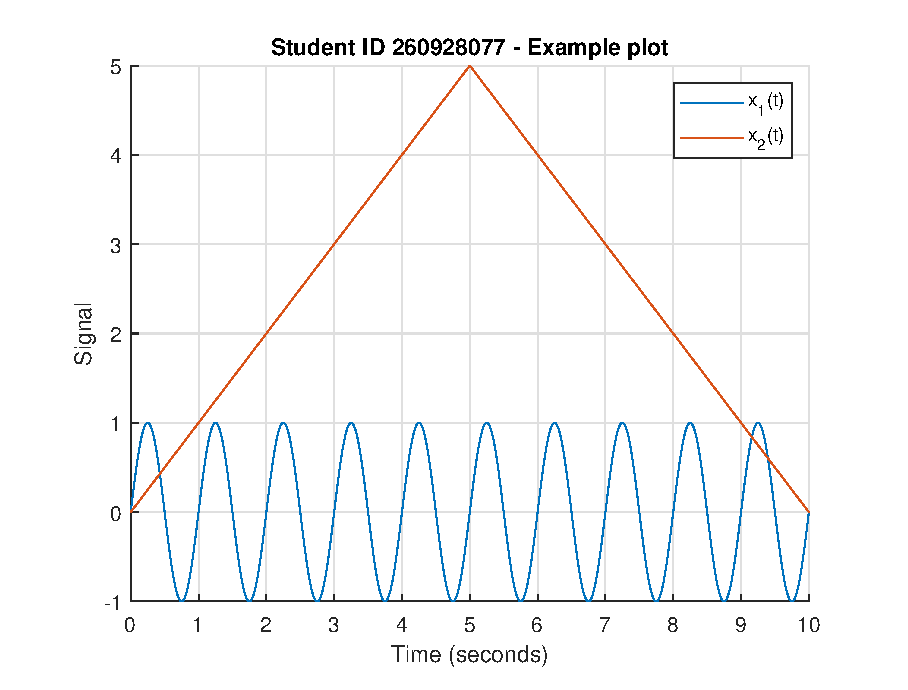
\includegraphics[width=\maxwidth{56.196688409433015em}]{figure_0.eps}
\end{center}


\matlabheading{\textit{2.4. Matrices in}\textit{ }\texttt{\textit{\textbf{MATLAB}}}}

\begin{par}
\begin{flushleft}
Matrices are extensions of arrays. They will be used to represent linear systems in a state space form.
\end{flushleft}
\end{par}

\begin{par}
\begin{flushleft}
For example to represent the matrix A:
\end{flushleft}
\end{par}

\begin{par}
$$A=\left(\begin{array}{ccc}
8 & 1 & 6\\
3 & 5 & 7\\
4 & 9 & 2
\end{array}\right)$$
\end{par}

\begin{par}
\begin{flushleft}
We write
\end{flushleft}
\end{par}

\begin{matlabcode}
A = [8, 1, 6; 3, 5, 7; 4, 9, 2]
\end{matlabcode}
\begin{matlaboutput}
A = 3x3    
     8     1     6
     3     5     7
     4     9     2

\end{matlaboutput}


\begin{par}
\begin{flushleft}
Determinant of A can be obtained by:
\end{flushleft}
\end{par}

\begin{matlabcode}
det(A)
\end{matlabcode}
\begin{matlaboutput}
ans = -360
\end{matlaboutput}


\begin{par}
\begin{flushleft}
Eigenvalues of A can be obtained by:
\end{flushleft}
\end{par}

\begin{matlabcode}
eig(A)
\end{matlabcode}
\begin{matlaboutput}
ans = 3x1    
   15.0000
    4.8990
   -4.8990

\end{matlaboutput}


\begin{par}
\begin{flushleft}
Inverse of A can be obtained by:
\end{flushleft}
\end{par}

\begin{matlabcode}
inv(A)
\end{matlabcode}
\begin{matlaboutput}
ans = 3x3    
    0.1472   -0.1444    0.0639
   -0.0611    0.0222    0.1056
   -0.0194    0.1889   -0.1028

\end{matlaboutput}


\matlabheading{\textit{2.5. Saving/loading data}}

\begin{par}
\begin{flushleft}
In \texttt{\textbf{MATLAB}} you can save any or all the variables in the current workspace to a MAT-file (.mat). You can then reuse the workspace variables later during the current MATLAB session or during another session by loading the saved MAT-file.
\end{flushleft}
\end{par}

\begin{par}
\begin{flushleft}
For example, to save a variable, you can use:
\end{flushleft}
\end{par}

\begin{matlabcode}
example = sprintf('A variable generated by Student ID <%s>', Students.ID);
save('Lab01.mat', 'example')
\end{matlabcode}


\begin{par}
\begin{flushleft}
Now we remove the variable \texttt{\textbf{example}} from the workspace.
\end{flushleft}
\end{par}

\begin{matlabcode}
clear example
\end{matlabcode}


\begin{par}
\begin{flushleft}
You can recover the variable \texttt{\textbf{example}} to the workspace from the MAT-file, by doing
\end{flushleft}
\end{par}

\begin{matlabcode}
load('Lab01.mat', 'example')
display(example)
\end{matlabcode}
\begin{matlaboutput}
example = 'A variable generated by Student ID <260928077>'
\end{matlaboutput}


\begin{par}
\begin{flushleft}
For hardware labs (labs that requires the use of external hardware), it is possible to save result of your manipulation in this manner. The resulting file can be used to re-examine your data, or change your plots.
\end{flushleft}
\end{par}

\matlabheading{\textit{Question 1 (4 marks)}}

\begin{par}
\begin{flushleft}
Answer the following questions in the LiveScript. (Observe that if you finish an expression with a semicolon the results will not show in your report. Use semicolons at the end of your expression with the intention to show or hide your answer)
\end{flushleft}
\end{par}

\begin{itemize}
\setlength{\itemsep}{-1ex}
   \item{\begin{flushleft} Define a time signal from 0 to 10 seconds, with a time step of 0.1 second. \end{flushleft}}
\end{itemize}

\begin{matlabcode}
dt = 0.1; % Timestemps of 0.1s of the discrete signal
T = 10; % Final value of time in seconds 
t = 0:dt:10 % Time signal
\end{matlabcode}
\begin{matlaboutput}
t = 1x101    
         0    0.1000    0.2000    0.3000    0.4000    0.5000    0.6000    0.7000    0.8000    0.9000    1.0000    1.1000    1.2000    1.3000    1.4000    1.5000    1.6000    1.7000    1.8000    1.9000    2.0000    2.1000    2.2000    2.3000    2.4000    2.5000    2.6000    2.7000    2.8000    2.9000    3.0000    3.1000    3.2000    3.3000    3.4000    3.5000    3.6000    3.7000    3.8000    3.9000    4.0000    4.1000    4.2000    4.3000    4.4000    4.5000    4.6000    4.7000    4.8000    4.9000

\end{matlaboutput}


\begin{itemize}
\setlength{\itemsep}{-1ex}
   \item{\begin{flushleft} Define a unit signal equals to 1 from 0 to 10 second. (The unit signal should have the same size as time) \end{flushleft}}
\end{itemize}

\begin{par}
$$y_1 (t)=1,~~t\ge 0$$
\end{par}

\begin{matlabcode}
y1 = ones(size(t)) % Create a 1 signal with the same size as time
\end{matlabcode}
\begin{matlaboutput}
y1 = 1x101    
     1     1     1     1     1     1     1     1     1     1     1     1     1     1     1     1     1     1     1     1     1     1     1     1     1     1     1     1     1     1     1     1     1     1     1     1     1     1     1     1     1     1     1     1     1     1     1     1     1     1

\end{matlaboutput}


\begin{itemize}
\setlength{\itemsep}{-1ex}
   \item{\begin{flushleft} Define a delayed signal equals zero from 0 to 5 seconds and to -1 from 5 to 10 seconds. \end{flushleft}}
\end{itemize}

\begin{par}
$$y_2 (t)=\left\lbrace \begin{array}{cc}
0, & t<5\\
-1, & t\ge 5
\end{array}\right.$$
\end{par}

\begin{matlabcode}
y2(t<5) = 0 % Case when t<5
\end{matlabcode}
\begin{matlaboutput}
y2 = 1x101    
     0     0     0     0     0     0     0     0     0     0     0     0     0     0     0     0     0     0     0     0     0     0     0     0     0     0     0     0     0     0     0     0     0     0     0     0     0     0     0     0     0     0     0     0     0     0     0     0     0     0

\end{matlaboutput}
\begin{matlabcode}
y2(t>=5) = -1 %Case when t>=5
\end{matlabcode}
\begin{matlaboutput}
y2 = 1x101    
     0     0     0     0     0     0     0     0     0     0     0     0     0     0     0     0     0     0     0     0     0     0     0     0     0     0     0     0     0     0     0     0     0     0     0     0     0     0     0     0     0     0     0     0     0     0     0     0     0     0

\end{matlaboutput}


\begin{itemize}
\setlength{\itemsep}{-1ex}
   \item{\begin{flushleft} Define a ramp signal with slope equals 0.1. \end{flushleft}}
\end{itemize}

\begin{par}
$$y_3 (t)=0.1t,~~t\ge 0$$
\end{par}

\begin{matlabcode}
y3(t>=0) = 0.1*t 
\end{matlabcode}
\begin{matlaboutput}
y3 = 1x101    
         0    0.0100    0.0200    0.0300    0.0400    0.0500    0.0600    0.0700    0.0800    0.0900    0.1000    0.1100    0.1200    0.1300    0.1400    0.1500    0.1600    0.1700    0.1800    0.1900    0.2000    0.2100    0.2200    0.2300    0.2400    0.2500    0.2600    0.2700    0.2800    0.2900    0.3000    0.3100    0.3200    0.3300    0.3400    0.3500    0.3600    0.3700    0.3800    0.3900    0.4000    0.4100    0.4200    0.4300    0.4400    0.4500    0.4600    0.4700    0.4800    0.4900

\end{matlaboutput}


\begin{itemize}
\setlength{\itemsep}{-1ex}
   \item{\begin{flushleft} Define a decaying exponential signal with time constant of 10 second. \end{flushleft}}
\end{itemize}

\begin{par}
$$y_4 (t)=e^{-\frac{t}{10}}$$
\end{par}

\begin{matlabcode}
y4 = 1*exp(-t/10) % Multiplication by 1 to convert symbolic function to numeric
\end{matlabcode}
\begin{matlaboutput}
y4 = 1x101    
    1.0000    0.9900    0.9802    0.9704    0.9608    0.9512    0.9418    0.9324    0.9231    0.9139    0.9048    0.8958    0.8869    0.8781    0.8694    0.8607    0.8521    0.8437    0.8353    0.8270    0.8187    0.8106    0.8025    0.7945    0.7866    0.7788    0.7711    0.7634    0.7558    0.7483    0.7408    0.7334    0.7261    0.7189    0.7118    0.7047    0.6977    0.6907    0.6839    0.6771    0.6703    0.6637    0.6570    0.6505    0.6440    0.6376    0.6313    0.6250    0.6188    0.6126

\end{matlaboutput}


\begin{itemize}
\setlength{\itemsep}{-1ex}
   \item{\begin{flushleft} Plot in the same graph the signals ($y_1 (t)$, $y_2 (t)$, $y_3 (t)$, and $y_4 (t)$) versus the time signal. \end{flushleft}}
\end{itemize}

\begin{matlabcode}
figure;
hold on;
grid on;
% Fill in your plots command

plot(t, y1);
plot(t, y2);
plot(t, y3);
plot(t, y4);

title(sprintf('Student ID %s - Question 1 - Signals', Students.ID));
xlabel('Time (seconds)')
ylabel('Signals')
legend('y_1(t)', 'y_2(t)', 'y_3(t)', 'y_4(t)', 'location', 'best')

hold off;
\end{matlabcode}
\begin{center}
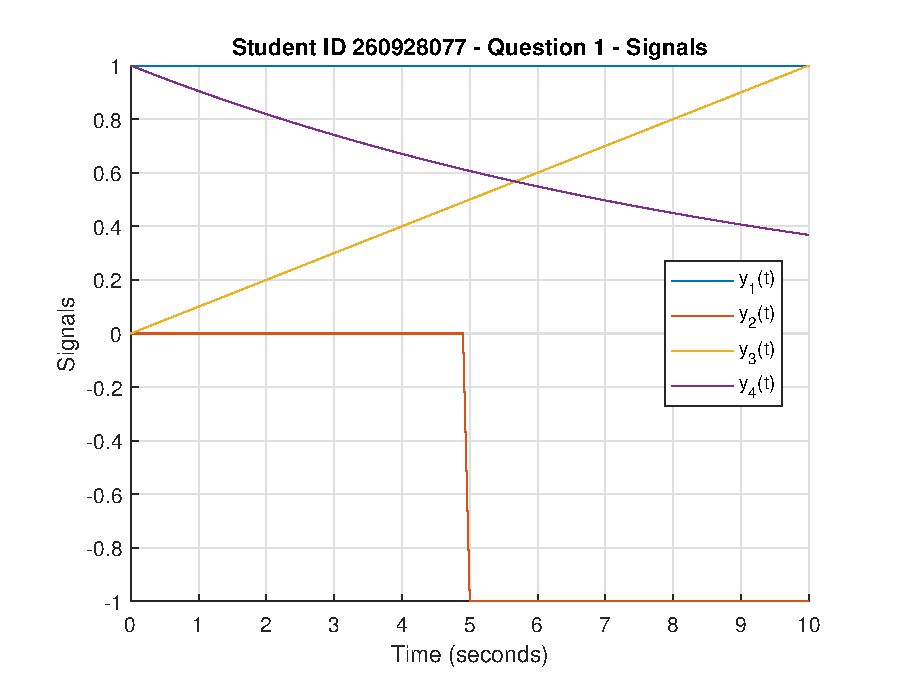
\includegraphics[width=\maxwidth{56.196688409433015em}]{figure_1.eps}
\end{center}


\matlabheading{\textbf{3. Laplace transforms}}

\begin{par}
\begin{flushleft}
Recall that the (one-sided) Laplace transform of a function $f(t)$ is defined as:
\end{flushleft}
\end{par}

\begin{par}
$$F(s)=\int_{0^- }^{+\infty } f(t)e^{-st} dt$$
\end{par}

\begin{par}
\begin{flushleft}
In this section, we will learn how to compute the Laplace and inverse Laplace transforms using \texttt{\textbf{MATLAB}}.
\end{flushleft}
\end{par}

\matlabheading{\textit{3.1. Computing Laplace Transform}}

\begin{par}
\begin{flushleft}
The command \texttt{\textbf{laplace}} in \texttt{\textbf{MATLAB}} provides an easy way to calculate the Laplace transform $F(s)$ of a function $f(t)$. To use \texttt{\textbf{laplace}}, first you need to specify that the variable $t$ and $s$ are symbolic ones. This is done with the command:
\end{flushleft}
\end{par}

\begin{matlabcode}
syms t s
\end{matlabcode}


\begin{par}
\begin{flushleft}
Then, we define the function $f(t)$.
\end{flushleft}
\end{par}

\begin{matlabcode}
f = exp(-t)
\end{matlabcode}
\begin{matlabsymbolicoutput}
f = 

\hskip1em $\displaystyle {\mathrm{e}}^{-t} $
\end{matlabsymbolicoutput}


\begin{par}
\begin{flushleft}
Finally, we compute the Laplace transform using the function \texttt{laplace}
\end{flushleft}
\end{par}

\begin{matlabcode}
F = laplace(f, t, s)
\end{matlabcode}
\begin{matlabsymbolicoutput}
F = 

\hskip1em $\displaystyle \frac{1}{s+1}$
\end{matlabsymbolicoutput}


\begin{par}
\begin{flushleft}
To get more information about the \texttt{\textbf{laplace}} function, type:
\end{flushleft}
\end{par}

\begin{matlabcode}
help laplace
\end{matlabcode}
\begin{matlaboutput}
--- help for sym/laplace ---

 laplace Laplace transform.
    L = laplace(F) is the Laplace transform of the sym F with default
    independent variable t.  The default return is a function of s.
    If F = F(s), then laplace returns a function of z:  L = L(z).
    By definition, L(s) = int(F(t)*exp(-s*t),t,0,inf).
 
    L = laplace(F,z) makes L a function of z instead of the default s:
    laplace(F,z) <=> L(z) = int(F(t)*exp(-z*t),t,0,inf).
 
    L = laplace(F,w,u) makes L a function of u instead of the
    default s (integration with respect to w).
    laplace(F,w,u) <=> L(u) = int(F(w)*exp(-u*w),w,0,inf).
 
    Examples:
     syms a s t w x F(t)
     laplace(t^5)          returns   120/s^6
     laplace(exp(a*s))     returns   -1/(a-z)
     laplace(sin(w*x),t)   returns   w/(t^2+w^2)
     laplace(cos(x*w),w,t) returns   t/(t^2+x^2)
     laplace(x^(3/2),t)    returns   (3*pi^(1/2))/(4*t^(5/2))
     laplace(diff(F(t)))   returns   s*laplace(F(t),t,s) - F(0)
 
    See also sym/ilaplace, sym/fourier, sym/htrans, sym/ztrans, subs.
\end{matlaboutput}


\begin{par}
\begin{flushleft}
Often, using \texttt{\textbf{laplace}} function gives an expression that is mathematically correct, but not in its simplest form. In such cases, the function \texttt{simplify} can be used to simplify the expression. For example:
\end{flushleft}
\end{par}

\begin{matlabcode}
simplify(2/(s + 1)-s/(s + 1)^2)
\end{matlabcode}
\begin{matlabsymbolicoutput}
ans = 

\hskip1em $\displaystyle \frac{s+2}{{{\left(s+1\right)}}^2 }$
\end{matlabsymbolicoutput}


\begin{par}
\begin{flushleft}
To get more information about the \texttt{\textbf{simplify}} function, type:
\end{flushleft}
\end{par}

\begin{matlabcode}
help sym/simplify
\end{matlabcode}
\begin{matlaboutput}
 simplify Symbolic simplification.
    simplify(S) simplifies each element of the symbolic matrix S.
    
    simplify(S,N) or, equivalently, simplify(S,'Steps',N),
    searches for a simplification in N steps. The default value of N is 1.
    
    simplify(S,'Seconds',T) aborts the search for a simpler version
    at the next end of a simplification step after T seconds. The results
    will depend on the speed and system load of your computer and may
    not be reproducible.
    
    simplify(S,'IgnoreAnalyticConstraints',VAL) controls the level of 
    mathematical rigor to use on the analytical constraints while simplifying 
    (branch cuts, division by zero, etc). The options for VAL are TRUE or 
    FALSE. Specify TRUE to relax the level of mathematical rigor
    in the rewriting process. The default is FALSE.
    
    simplify(S, 'Criterion', 'preferReal') 
    discourages simplify from returning results 
    containing complex numbers.
 
    simplify(S, 'All', true) 
    returns a column vector of aquivalent results. Typically used in
    combination with 'Steps', N.
 
    Examples: 
       syms x c alpha beta
 
       simplify(sin(x)^2 + cos(x)^2)  returns  1.
       simplify(exp(c*log(sqrt(alpha+beta))))  returns  (alpha + beta)^(c/2).
       simplify(sqrt(x^2))  returns  sqrt(x^2),
       simplify(sqrt(x^2),'IgnoreAnalyticConstraints',true)  returns  x.
       u = symunit;
       simplify(u.m+u.mm) returns  (1001/1000)*[m].
 
    See also symunit, sym/factor, sym/expand, sym/collect.
\end{matlaboutput}


\matlabheading{\textit{Question 2 (2 marks)}}

\begin{par}
\begin{flushleft}
Write the symbolic expression of the following functions (you can use the symbolic variables \texttt{\textbf{t}} and \texttt{\textbf{s}} defined previously):
\end{flushleft}
\end{par}

\begin{enumerate}
\setlength{\itemsep}{-1ex}
   \item{\begin{flushleft} $f_1 (t)=\delta (t)$ ($\delta (t)$ is the dirac function, use \texttt{\textbf{help dirac}} for more information) \end{flushleft}}
   \item{\begin{flushleft} $\displaystyle f_2 (t)=t^2 +4t+1$ \end{flushleft}}
   \item{\begin{flushleft} $\displaystyle f_3 (t)=te^{-t} +0.5e^{-t} +e^{-3t}$ \end{flushleft}}
   \item{\begin{flushleft} $\displaystyle f_4 (t)=\sin (2t)+\cos^2 (t)$ \end{flushleft}}
   \item{\begin{flushleft} $\displaystyle f_5 (t)=e^{-t} \sin (5t+\frac{\pi }{3})+t^2 e^{-2t}$ \end{flushleft}}
\end{enumerate}

\begin{matlabcode}
f1 = dirac(t)
\end{matlabcode}
\begin{matlabsymbolicoutput}
f1 = 

\hskip1em $\displaystyle {\delta }\left(t\right)$
\end{matlabsymbolicoutput}
\begin{matlabcode}
f2 = (t.^2)+(4*t)+1
\end{matlabcode}
\begin{matlabsymbolicoutput}
f2 = 

\hskip1em $\displaystyle t^2 +4\,t+1$
\end{matlabsymbolicoutput}
\begin{matlabcode}
f3 = (t*exp(-t))+(0.5*exp(-t))+(exp(-3*t))
\end{matlabcode}
\begin{matlabsymbolicoutput}
f3 = 

\hskip1em $\displaystyle \frac{{\mathrm{e}}^{-t} }{2}+{\mathrm{e}}^{-3\,t} +t\,{\mathrm{e}}^{-t} $
\end{matlabsymbolicoutput}
\begin{matlabcode}
f4 = sin(2*t)+cos(t).^2
\end{matlabcode}
\begin{matlabsymbolicoutput}
f4 = 

\hskip1em $\displaystyle {\cos \left(t\right)}^2 +\sin \left(2\,t\right)$
\end{matlabsymbolicoutput}
\begin{matlabcode}
f5 = exp(-t)*sin(5*t+pi/3)+t.^2*exp(-2*t)
\end{matlabcode}
\begin{matlabsymbolicoutput}
f5 = 

\hskip1em $\displaystyle t^2 \,{\mathrm{e}}^{-2\,t} +\sin \left(5\,t+\frac{\pi }{3}\right)\,{\mathrm{e}}^{-t} $
\end{matlabsymbolicoutput}


\matlabheading{\textit{Question 3 (2 marks)}}

\begin{par}
\begin{flushleft}
Use \texttt{\textbf{MATLAB}} to compute the Laplace transform of the functions defined in \textit{Question 2}. Use \texttt{\textbf{simplify}} to simplify the symbolic expression if needed.
\end{flushleft}
\end{par}

\begin{matlabcode}
F1 = laplace(f1, t, s)
\end{matlabcode}
\begin{matlabsymbolicoutput}
F1 = 

\hskip1em $\displaystyle 1$
\end{matlabsymbolicoutput}
\begin{matlabcode}
F2 = simplify(laplace(f2, t, s))
\end{matlabcode}
\begin{matlabsymbolicoutput}
F2 = 

\hskip1em $\displaystyle \frac{s^2 +4\,s+2}{s^3 }$
\end{matlabsymbolicoutput}
\begin{matlabcode}
F3 = simplify(laplace(f3, t, s))
\end{matlabcode}
\begin{matlabsymbolicoutput}
F3 = 

\hskip1em $\displaystyle \frac{3\,s^2 +10\,s+11}{2\,{{\left(s+1\right)}}^2 \,{\left(s+3\right)}}$
\end{matlabsymbolicoutput}
\begin{matlabcode}
F4 = simplify(laplace(f4, t, s))
\end{matlabcode}
\begin{matlabsymbolicoutput}
F4 = 

\hskip1em $\displaystyle \frac{s^2 +2\,s+2}{s\,{\left(s^2 +4\right)}}$
\end{matlabsymbolicoutput}
\begin{matlabcode}
F5 = simplify(laplace(f5, t, s))
\end{matlabcode}
\begin{matlabsymbolicoutput}
F5 = 

\hskip1em $\displaystyle \frac{2}{{{\left(s+2\right)}}^3 }+\frac{5}{2\,{\left({{\left(s+1\right)}}^2 +25\right)}}+\frac{\sqrt{3}\,{\left(s+1\right)}}{2\,{\left({{\left(s+1\right)}}^2 +25\right)}}$
\end{matlabsymbolicoutput}


\matlabheading{\textit{3.2. Computing inverse Laplace transforms}}

\begin{par}
\begin{flushleft}
The function \texttt{\textbf{ilaplace}} computes the inverse Laplace transform. Consider the Laplace transform \texttt{\textbf{F}} computed earlier. We can compute the inverse Laplace transform (note that the \texttt{\textbf{t}} and \texttt{\textbf{s}} are already defined as symbols)
\end{flushleft}
\end{par}

\begin{par}
\begin{flushleft}
Example
\end{flushleft}
\end{par}

\begin{matlabcode}
ilaplace(F, s, t);
\end{matlabcode}


\matlabheading{\textit{Question 4 (2 marks)}}

\begin{par}
\begin{flushleft}
Use \texttt{\textbf{MATLAB}} to calculate the inverse Laplace transform of the following expressions. Use \texttt{\textbf{simplify}} to simplify the symbolic expression if needed.
\end{flushleft}
\end{par}

\begin{enumerate}
\setlength{\itemsep}{-1ex}
   \item{\begin{flushleft} $\displaystyle G_1 (s)={{\frac{1}{s}}}$ \end{flushleft}}
   \item{\begin{flushleft} $\displaystyle G_2 (s)={{\frac{1}{s(s+1)}}}$ \end{flushleft}}
   \item{\begin{flushleft} $\displaystyle G_3 (s)={{\frac{5}{s^2 +25}}}$ \end{flushleft}}
   \item{\begin{flushleft} $\displaystyle G_4 (s)={{\frac{10s+1}{s^2 +2s+10}}}$ \end{flushleft}}
   \item{\begin{flushleft} $\displaystyle G_5 (s)={{\frac{2(s+1)(s^2 +4)}{(s^2 +4s+1)(s^2 +9)}}}$ \end{flushleft}}
\end{enumerate}

\begin{matlabcode}
G1 = 1/s
\end{matlabcode}
\begin{matlabsymbolicoutput}
G1 = 

\hskip1em $\displaystyle \frac{1}{s}$
\end{matlabsymbolicoutput}
\begin{matlabcode}
G2 = 1/(s*(s+1))
\end{matlabcode}
\begin{matlabsymbolicoutput}
G2 = 

\hskip1em $\displaystyle \frac{1}{s\,{\left(s+1\right)}}$
\end{matlabsymbolicoutput}
\begin{matlabcode}
G3 = 5/(s.^2+25)
\end{matlabcode}
\begin{matlabsymbolicoutput}
G3 = 

\hskip1em $\displaystyle \frac{5}{s^2 +25}$
\end{matlabsymbolicoutput}
\begin{matlabcode}
G4 = (10*s+1)/(s.^2+2*s+10)
\end{matlabcode}
\begin{matlabsymbolicoutput}
G4 = 

\hskip1em $\displaystyle \frac{10\,s+1}{s^2 +2\,s+10}$
\end{matlabsymbolicoutput}
\begin{matlabcode}
G5 = (2*(s+1)*(s.^2+4))/(((s.^2)+4*s+1)*(s.^2+9))
\end{matlabcode}
\begin{matlabsymbolicoutput}
G5 = 

\hskip1em $\displaystyle \frac{{\left(2\,s+2\right)}\,{\left(s^2 +4\right)}}{{\left(s^2 +9\right)}\,{\left(s^2 +4\,s+1\right)}}$
\end{matlabsymbolicoutput}
\begin{matlabcode}

g1 = ilaplace(G1, s, t)
\end{matlabcode}
\begin{matlabsymbolicoutput}
g1 = 

\hskip1em $\displaystyle 1$
\end{matlabsymbolicoutput}
\begin{matlabcode}
g2 = ilaplace(G2, s, t)
\end{matlabcode}
\begin{matlabsymbolicoutput}
g2 = 

\hskip1em $\displaystyle 1-{\mathrm{e}}^{-t} $
\end{matlabsymbolicoutput}
\begin{matlabcode}
g3 = ilaplace(G3, s, t)
\end{matlabcode}
\begin{matlabsymbolicoutput}
g3 = 

\hskip1em $\displaystyle \sin \left(5\,t\right)$
\end{matlabsymbolicoutput}
\begin{matlabcode}
g4 = ilaplace(G4, s, t)
\end{matlabcode}
\begin{matlabsymbolicoutput}
g4 = 

\hskip1em $\displaystyle 10\,{\mathrm{e}}^{-t} \,{\left(\cos \left(3\,t\right)-\frac{3\,\sin \left(3\,t\right)}{10}\right)}$
\end{matlabsymbolicoutput}
\begin{matlabcode}
g5 = ilaplace(G5, s, t)
\end{matlabcode}
\begin{matlabsymbolicoutput}
g5 = 

\hskip1em $\displaystyle \frac{15\,\cos \left(3\,t\right)}{26}-\frac{35\,\sin \left(3\,t\right)}{78}+\frac{37\,{\mathrm{e}}^{-2\,t} \,{\left(\cosh \left(\sqrt{3}\,t\right)-\frac{47\,\sqrt{3}\,\sinh \left(\sqrt{3}\,t\right)}{111}\right)}}{26}$
\end{matlabsymbolicoutput}

\end{document}
